\documentclass[12pt]{article}
\usepackage{amsmath}
\usepackage{amssymb}
\usepackage{xcolor}
\usepackage{tikz}
\usepackage[colorlinks]{hyperref}

\newcommand{\calR}{\mathcal{R}}

\newcommand{\calS}{\mathcal{S}}

\newcommand{\calL}{\mathcal{L}}

\newcommand{\calX}{\mathcal{X}}

\newcommand{\calE}{\mathcal{E}}

\begin{document}

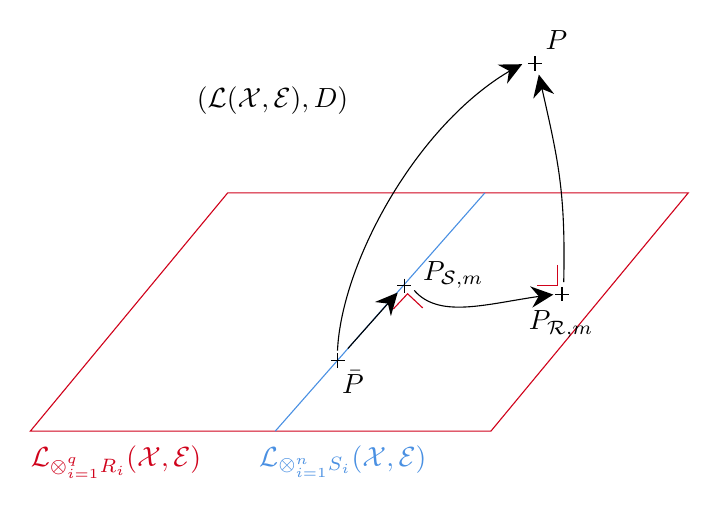
\begin{tikzpicture}[x=0.75pt,y=0.75pt,yscale=-1,xscale=1]

\draw  [color={rgb, 255:red, 208; green, 2; blue, 27 }  ,draw opacity=1 ] (216.1,134.33) -- (438,134.33) -- (342.9,249.14) -- (121,249.14) -- cycle ;
\draw [color={rgb, 255:red, 74; green, 144; blue, 226 }  ,draw opacity=1 ]   (340,134.33) -- (239,249.14) ;
\draw   (265.69,215.08) -- (272.64,215.08)(269.17,211.61) -- (269.17,218.56) ;
\draw   (373.69,183.08) -- (380.64,183.08)(377.17,179.61) -- (377.17,186.56) ;
\draw   (297.69,179.08) -- (304.64,179.08)(301.17,175.61) -- (301.17,182.56) ;
\draw   (360.69,72.08) -- (367.64,72.08)(364.17,68.61) -- (364.17,75.56) ;
\draw    (269,210.33) .. controls (270.97,166.99) and (308.84,98.43) .. (355.85,73.44) ;
\draw [shift={(358,72.33)}, rotate = 153.43] [fill={rgb, 255:red, 0; green, 0; blue, 0 }  ][line width=0.08]  [draw opacity=0] (10.72,-5.15) -- (0,0) -- (10.72,5.15) -- (7.12,0) -- cycle    ;
\draw    (378,177.33) .. controls (378.98,132.25) and (375.16,117.91) .. (366.53,79.7) ;
\draw [shift={(366,77.33)}, rotate = 77.32] [fill={rgb, 255:red, 0; green, 0; blue, 0 }  ][line width=0.08]  [draw opacity=0] (10.72,-5.15) -- (0,0) -- (10.72,5.15) -- (7.12,0) -- cycle    ;
\draw    (306,181.33) .. controls (318.55,195.81) and (343.2,187) .. (370.07,183.67) ;
\draw [shift={(373,183.33)}, rotate = 173.88] [fill={rgb, 255:red, 0; green, 0; blue, 0 }  ][line width=0.08]  [draw opacity=0] (10.72,-5.15) -- (0,0) -- (10.72,5.15) -- (7.12,0) -- cycle    ;
\draw  [color={rgb, 255:red, 208; green, 2; blue, 27 }  ,draw opacity=1 ] (295.93,190.24) -- (302.76,182.93) -- (310.07,189.76) ;
\draw  [color={rgb, 255:red, 208; green, 2; blue, 27 }  ,draw opacity=1 ] (375,169) -- (375,179) -- (365,179) ;
\draw    (274,209.33) -- (296.01,184.58) ;
\draw [shift={(298,182.33)}, rotate = 131.63] [fill={rgb, 255:red, 0; green, 0; blue, 0 }  ][line width=0.08]  [draw opacity=0] (10.72,-5.15) -- (0,0) -- (10.72,5.15) -- (7.12,0) -- cycle    ;

% Text Node
\draw (368,55) node [anchor=north west][inner sep=0.75pt]   [align=left] {$P$};
% Text Node
\draw (270,219) node [anchor=north west][inner sep=0.75pt]   [align=left] {$\bar{P}$};
% Text Node
\draw (360,190) node [anchor=north west][inner sep=0.75pt]   [align=left] {$P_{\calR, m}$};
% Text Node
\draw (309,166) node [anchor=north west][inner sep=0.75pt]   [align=left] {$P_{\calS, m}$};
% Text Node
\draw (200,82) node [anchor=north west][inner sep=0.75pt]   [align=left] {$(\calL(\calX, \calE), D)$};
% Text Node
\draw (120,255) node [anchor=north west][inner sep=0.75pt]  [color={rgb, 255:red, 208; green, 2; blue, 27 }  ,opacity=1 ] [align=left] {$\calL_{\otimes_{i=1}^{q} R_i}(\calX, \calE)$};
% Text Node
\draw (230,255) node [anchor=north west][inner sep=0.75pt]  [color={rgb, 255:red, 74; green, 144; blue, 226 }  ,opacity=1 ] [align=left] {$\calL_{\otimes_{i=1}^{n} S_i}(\calX, \calE)$};


\end{tikzpicture}

\end{document}